%NYU 2019 Grad Computational Physics Homework 4

\documentclass[12pt, graphicx]{article}
\pagestyle{plain}
\baselineskip 18pt
\textwidth 6.5in
\textheight 7.8in
\oddsidemargin 0.1in
\evensidemargin 0.1in
\topmargin 0.3in
\parindent 0pt
\linespread{1.5}
\setlength{\parskip}{2.5mm}

\usepackage{graphicx, psfrag, epsfig}
\usepackage[font = small, format = plain, labelfont = bf, textfont = it, justification = raggedright, singlelinecheck = false]{caption}
\usepackage{subfig}
\usepackage{amsmath, amssymb}
\usepackage{geometry}
%\usepackage[symbol]{footmisc}

\renewcommand\tablename{Table}
\renewcommand\figurename{Fig.}
\renewcommand{\thefootnote}{\fnsymbol{footnote}}


\begin{document}
\title{Computational Physics Homework 4}
\author{Hao Li\footnotemark[2]}
\footnotetext[2]{hl3270@nyu.edu~~UID:N12137527}
\date{\today}


\maketitle

\section*{Problem 1}
The equations for the Brusselator:
\begin{equation}
\begin{gathered}
\frac{\mathrm{d}x}{\mathrm{d}t}=1-(b+1)x+ax^2y\\
\frac{\mathrm{d}y}{\mathrm{d}t}=bx-ax^2y
\end{gathered}
\label{eq:bru}
\end{equation}
Here we choose $a=1$, $b=3$, initial condition $x=y=0$, and time interval $t=0\to t=H=20$.\par
To prove the accuracy of our following solutions, first calculate using modified midpoint method with fixed small step size $h=0.01$, and for all steps, $n=8$. The plot of the result for the concentration of chemicals in this method is shown as Fig. \ref{fig:bru_mod}, we can see $x,y$ soon converge to oscillation. 

\begin{figure}[ht]
\centering
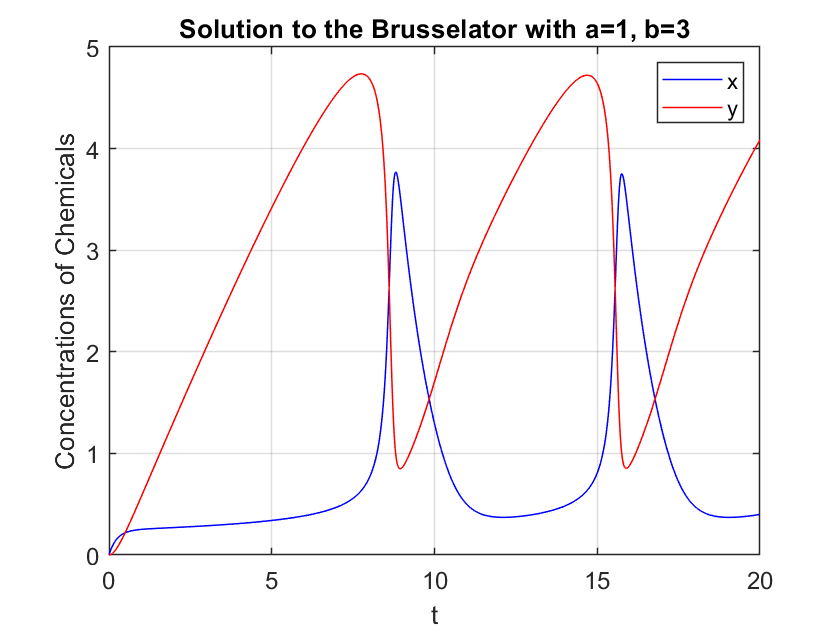
\includegraphics[width = 120mm]{Brusselator_mod_mid.png}
\caption{The solution to the equation of Brusselator Eq. \ref{eq:bru} using modified midpoint method. Parameters are chosen to be $a=1$, $b=3$, initial condition $x=y=0$, and time interval $t=0\to t=H=20$. Step sizes are the same $h=0.01$, small enough to get the accurate solution. Clear oscillation can be noticed from the plot.}
\label{fig:bru_mod}
\end{figure}

Then we change into adaptive Bulirsch-Stoer method, where we both change the step sizes and the value of $n$ for each step. Accuracy is set to be $\delta=10^{-10}$, so we will keep bisecting the present interval until the error Eq. \ref{eq:bru_err} for $m=n-1$, given in the textbook, is better than the the target accuracy $h_i\delta$, where $h_i$ is the the stepsize of the next interval. For each interval, the maximum of $n=8$. Once reaching the target accuracy, we will move to the next interval.
\begin{equation}
\epsilon=\frac{R_{n,m}-R_{n-1,m}}{[n/(n-1)]^{2m}-1}
\label{eq:bru_err}
\end{equation}
The result of the adaptive Bulirsch-Stoer method for Eq. \ref{eq:bru} is given in Fig. \ref{fig:bur_BS}. In this plot, it is obvious that arround the peaks of variable $x$, points are significantly closer, i.e. $x\approx[7.5,10],[15,17.5]$. 

\begin{figure}[ht]
\centering
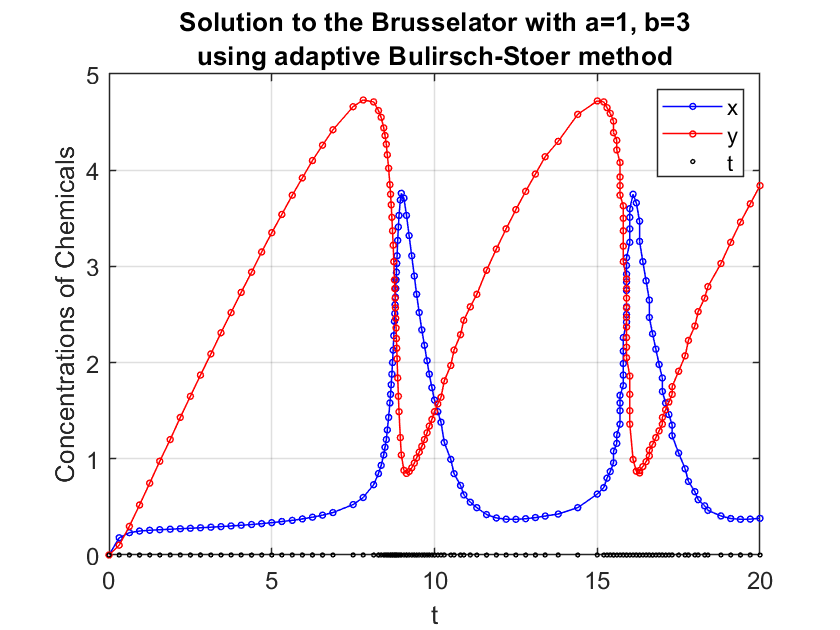
\includegraphics[width = 120mm]{Brusselator_BS.png}
\caption{The solution to the equation of Brusselator Eq. \ref{eq:bru} using adaptive Bulirsch-Stoer method. Parameters are chosen to be $a=1$, $b=3$, initial condition $x=y=0$, and time interval $t=0\to t=H=20$. We start with a single step, i.e. $h_0=H$. From this plot, we can infer that points are significantly closer at $x\approx[7.5,10],[15,17.5]$, where $x$ changes rapidly. Arround these values, we will need much smaller step size to allow higher accuracy.}
\label{fig:bru_BS}
\end{figure}

\section*{Problem 2}
\subsection*{a)}
The code for adaptive time step RK4 method is available in \textquotedblleft ODE.h\textquotedblright. \par
For this problem, the equation of motion for one black hole in a supermassive black hole binary (SBHB) is 
\begin{equation}
\frac{\mathrm{d}^2\mathbf{r}_{BH}}{\mathrm{d}t^2}=-\frac{GM_{BH}}{4r^3_{BH}}\mathbf{r}_{BH}+\dot{\mathbf{v}}_{DF}
\end{equation}
with approximate friction term given by
\begin{equation}
\dot{\mathbf{v}}_{DF}=-\frac{A}{v^3_{BH}+B}\mathbf{v}_{BH}
\end{equation}
Therefore, combine these two equations and take the velocity as an independent variable, we will get equations of a similar type of Prob. 1
\begin{equation}
\begin{gathered}
\frac{\mathrm{d}\mathbf{r}_{BH}}{\mathrm{d}t}=\mathbf{v}_{BH}\\
\frac{\mathrm{d}\mathbf{v}_{BH}}{\mathrm{d}t}=-\frac{GM_{BH}}{4r^3_{BH}}\mathbf{r}_{BH}-\frac{A}{v^3_{BH}+B}\mathbf{v}_{BH}
\end{gathered}
\label{eq:SBHB}
\end{equation}
Define the new four dimensional independent variable as $\mathbf{r}=(x_{BH}, y_{BH}, v_{x,BH}, v_{y,BH})$, then Eq. \ref{eq:SBHB} can be writen in the form
\begin{equation}
\frac{\mathrm{d}\mathbf{r}}{\mathrm{d}t}=\mathbf{f}(\mathbf{r},t)
\end{equation}
In this way, we can use Runge-Kutta method for multi-dimension to calculate the next point, as given in the book. To save time and get higher accuracy, we use RK4 method with adaptive time steps to solve the orbits. As given at page 358, we usually start with a small stepsize $h$, $\mathbf{r}_1$ and $\mathbf{r}_2$ are respectively the result for $t+2h$, calculated with two small steps $h$ and one large step $2h$. The next time step $h'$ is calculated by
\begin{equation}
h'=h\rho^{1/4}
\label{eq:h'}
\end{equation}
where
\begin{equation}
\rho=\frac{30h\delta}{|\mathbf{r}_1-\mathbf{r}_2|}
\label{eq:rho}
\end{equation}
Here $\delta$ is exactly the error tolerance per unit time. When $\rho\geq1$, $\mathbf{r}_1$ is chosen to be the next point. No matter it is true or not, we will always refresh the time step with Eq. \ref{eq:h'}. We will stop when reaching the final time or other conditions. In this problem, we only use the position parts of the variables in Eq. \ref{eq:rho}. If consider all the four components, the program will breakdown near the origin in part a), since the value and error of velocity is large near the origin, so $\rho$ will keep getting smaller until overflow.\par
Now we already have the mothod to use, then we will find an optimal value for $\delta$. Without dynamical friction, the equation is just the ordinary equation of motion in gravatity. Since total energy and angular momentum are reserved in this case, for the two side points of the ecllipse orbit, we have
\begin{equation}
\begin{gathered}
\frac{1}{2}v_1^2-\frac{1}{2}\frac{GM}{2r_1}=\frac{1}{2}v_2^2-\frac{1}{2}\frac{GM}{2r_2}\\
v_1r_1=v_2r_2
\end{gathered}
\label{eq:v1}
\end{equation}
Since we set $M=G=1$, $r_1=1$, $r_2=r_S=10^{-7}$, the Schwarzschild radius, plug them into Eq. \ref{eq:v1}, and we will get the initial velocity
\begin{equation}
v_0=\sqrt{\frac{1}{2(10^7+1)}}\approx2.236\times10^{-4}
\end{equation}
Calculating the orbits with this initial velosity $\mathbf{v}_0=(0,2.236\times10^{-4})$, initial position $x=1$, $y=0$, and different $\delta$, we get the following results. Three different $\delta=10^{-6}, 10^{-7}, 10^{-8}$ are chosen to show the accuracy. From Fig. \ref{fig:BHa}, we can see that for $\delta=10^{-6}$, there is an obvious loss of accuracy far from the origin. For $\delta=10^{-7}, 10^{-8}$, there are both no appreciable loss of accuracy, but still $\delta=10^{-8}$ is much better which we will use in the following calculation. To view more clearly, we can see in Fig. \ref{fig:BHar} that for $\delta=10^{-6}$, the radius at the far end is keep increasing noticibly, while for $\delta=10^{-8}$, the orbit is nearly exactly periodic. Additionally, $\log(r)$ is also plotted with respect to time, from which Fig. \ref{fig:BHalogr} we notice that $r_\mathrm{peri}$ stays perfectly arround $r_S=10^{-7}$ after 10 orbits.\par
Moreover, From unit analysis, we have
\begin{equation}
[T]=\sqrt{\frac{[D]^3}{[G][M]}}
\end{equation}
In this problem, we set $[D]=100\mathrm{pc}=3.0857\times10^{18}\mathrm{m}$, $G=6.67408\times10^{-11}\mathrm{m^3/(kg\cdot s^2)}=1$, $M=10^8M_\odot=1.98847\times10^{38}\mathrm{kg}$, one year has $31,557,600\mathrm{s}$, therefore, the unit of time is
\begin{equation}
[T]=4.7052\times10^{13}\mathrm{s}\approx1.49(1)\mathrm{Myr}
\end{equation}

\begin{figure}[ht]
\begin{minipage}{0.48\linewidth}
\centering
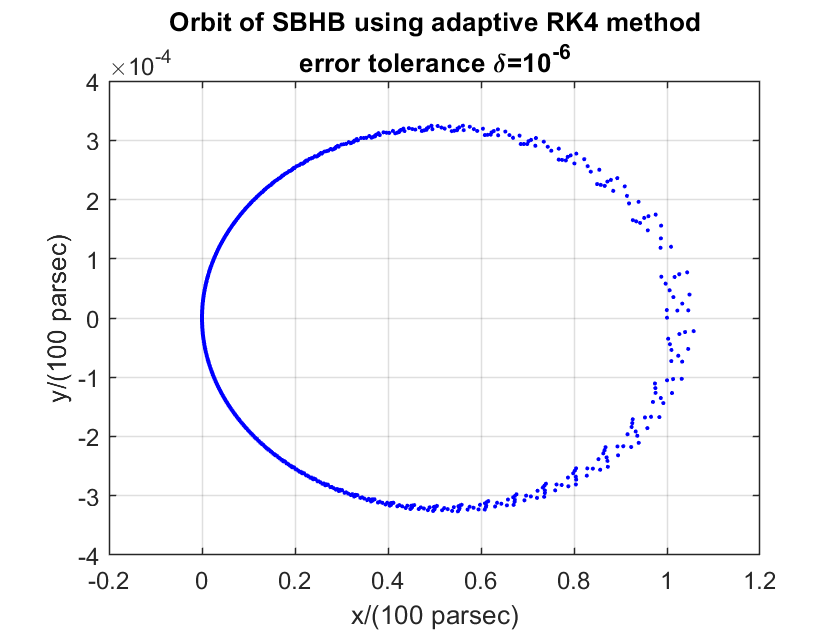
\includegraphics[width = 80mm]{BH_a6.png}
\end{minipage}
\begin{minipage}{0.48\linewidth}
\centering
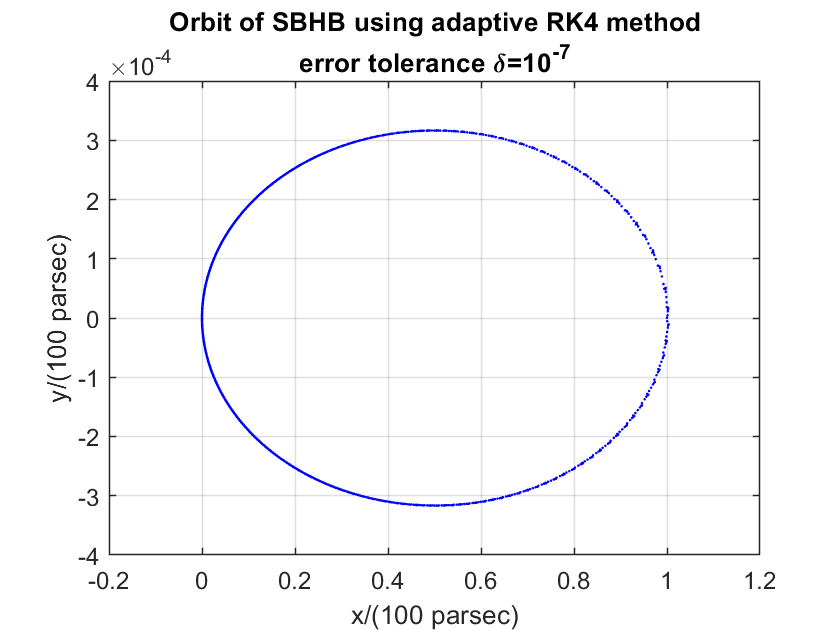
\includegraphics[width = 80mm]{BH_a7.png}
\end{minipage}
\centering
\begin{minipage}{0.48\linewidth}
\centering
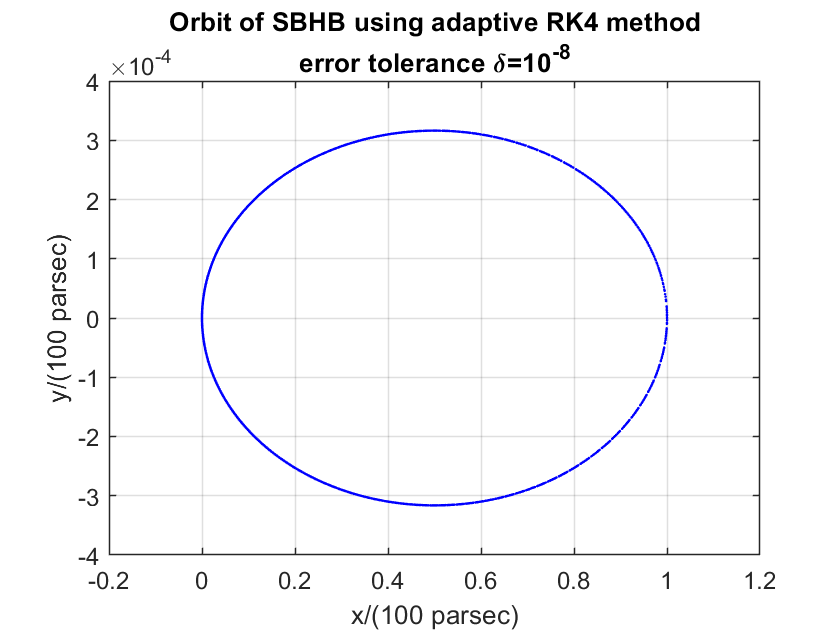
\includegraphics[width = 80mm]{BH_a8.png}
\end{minipage}
\caption{The orbits of supermassive black hole binary without dynamical friction using adaptive time step fourth-order Runge-Kutta method. Initial position $x=1$, $y=0$, targer time range $H=50$. Initial velosity $\mathbf{v}_0=(0,2.236\times10^{-4})$ so that the pericenter radius $r_\mathrm{peri}=r_S=10^{-7}$ is the Schwartzschild radius. Three different  $\delta=10^{-6}, 10^{-7}, 10^{-8}$ are chosen to show the accuracy. From the plots, we can clearly notice a significant loss of accuracy for $\delta=10^{-6}$, that the orbit is getting larger, which conflicts with the energy reserving condition. $\delta=10^{-7}$ is already good enough, but still $\delta=10^{-8}$ looks even smoother. }
\label{fig:BHa}
\end{figure}

\begin{figure}[ht]
\begin{minipage}{0.48\linewidth}
\centering
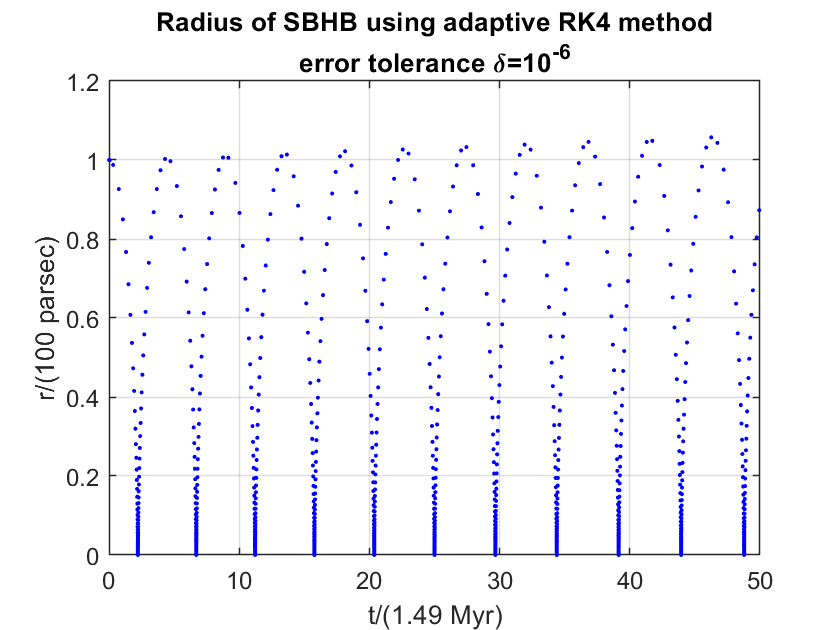
\includegraphics[width = 80mm]{BH_a6r.png}
\end{minipage}
\begin{minipage}{0.48\linewidth}
\centering
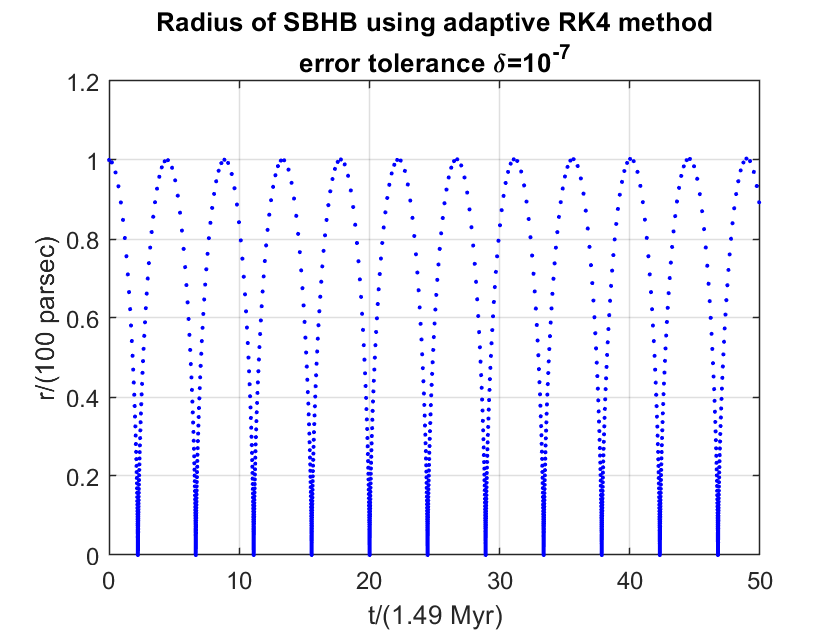
\includegraphics[width = 80mm]{BH_a7r.png}
\end{minipage}
\centering
\begin{minipage}{0.48\linewidth}
\centering
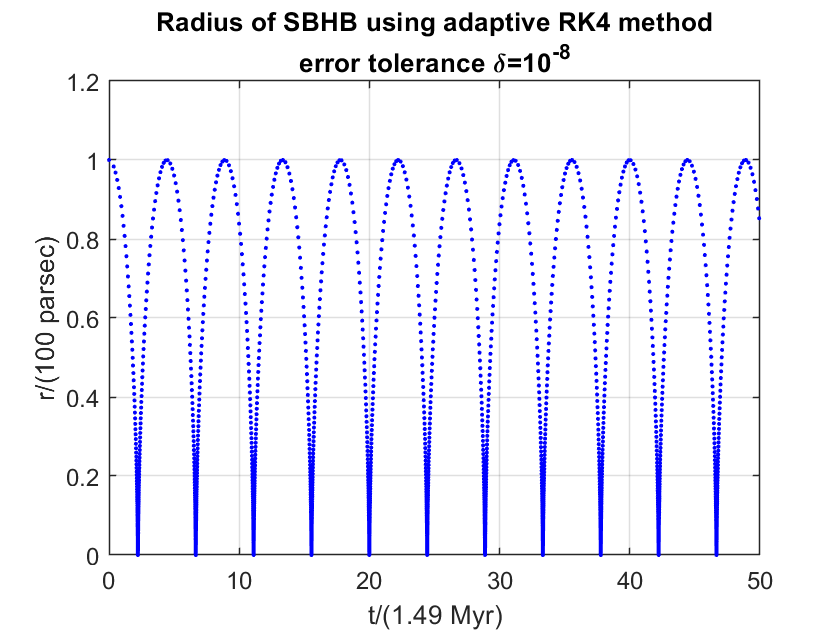
\includegraphics[width = 80mm]{BH_a8r.png}
\end{minipage}
\caption{The radius of the orbits of supermassive black hole binary without dynamical friction using adaptive time step fourth-order Runge-Kutta method. Initial position $x=1$, $y=0$, target time range $H=50$. Initial velosity $\mathbf{v}_0=(0,2.236\times10^{-4})$ so that the pericenter radius $r_\mathrm{peri}=r_S=10^{-7}$ is the Schwartzschild radius. Three different  $\delta=10^{-6}, 10^{-7}, 10^{-8}$ are chosen to show the accuracy. From the plots, we can notice that the maximum radius of each cycle has a significant increase for $\delta=10^{-6}$, while just as seen in Fig. \ref{fig:BHa}, the radius of each cycle of the orbit stays nearly the same for the other two, indicating that there is no appreciable loss of accuracy over 10 orbits. To get smoother results, we choose $\delta=10^{-8}$ for the following calculations.}
\label{fig:BHar}
\end{figure}

\clearpage

\begin{figure}[ht]
\centering
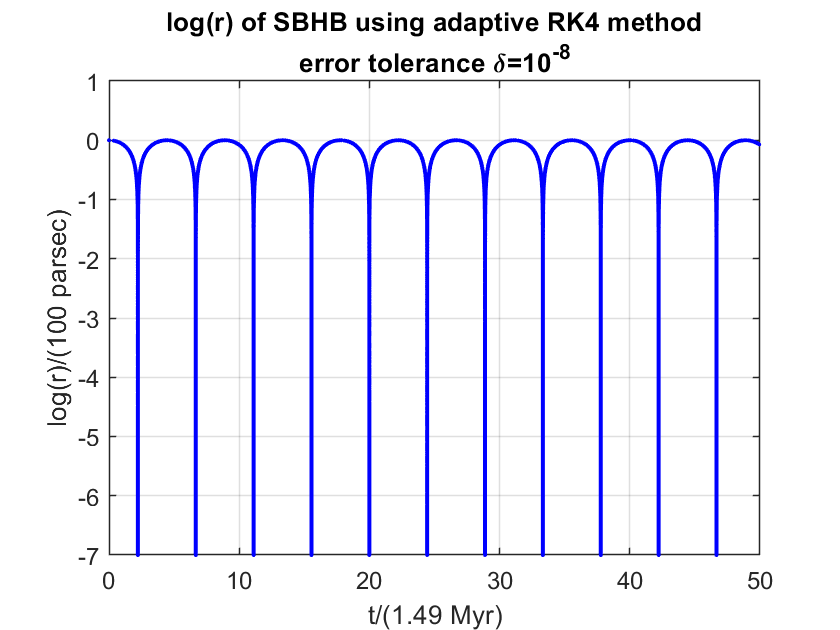
\includegraphics[width = 100mm]{BH_a8logr.png}
\caption{Logarithm of radius of the orbit of supermassive black hole binary without dynamical friction using adaptive time step fourth-order Runge-Kutta method. Initial position $x=1$, $y=0$, targer time range $H=50$. Initial velosity $\mathbf{v}_0=(0,2.236\times10^{-4})$ so that the pericenter radius $r_\mathrm{peri}=r_S=10^{-7}$ is the Schwartzschild radius. Error tolerance per unit time $\delta=10^{-8}$. The minimum of radius, i.e. the perimeter radius stays perfectly arround $r_S=10^{-7}$, we can imply from this plot. Therefore, there is no appreciable loss of accuracy over 10 orbits for $\delta=10^{-8}$ we are going to use.}
\label{fig:BHalogr}
\end{figure}

\subsection*{b)}
Now we add dynamical friction to the equation of motion.\par
First calculate the initial velocity. For circular orbit, we have
\begin{equation}
\frac{v^2}{r}=\frac{GM}{(2r)^2}
\end{equation}
The velocity for the circular orbit is
\begin{equation}
v=\frac{1}{2}\sqrt{\frac{GM}{r}}=0.5
\end{equation}
Therefore, the initial velocity for part b) is $v_0=0.8v=0.4$. Similar to the calculation of the unit of time, the unit of velocity is $[v]=\sqrt{\frac{[G][M]}{[D]}}=65.6\mathrm{km/s}$. Plug it in the program, and change the stop condition as the radius reaching the Schwarzschild radius, we get the following result, plotted in Fig. \ref{fig:BHb}. 

\begin{figure}[ht]
\centering
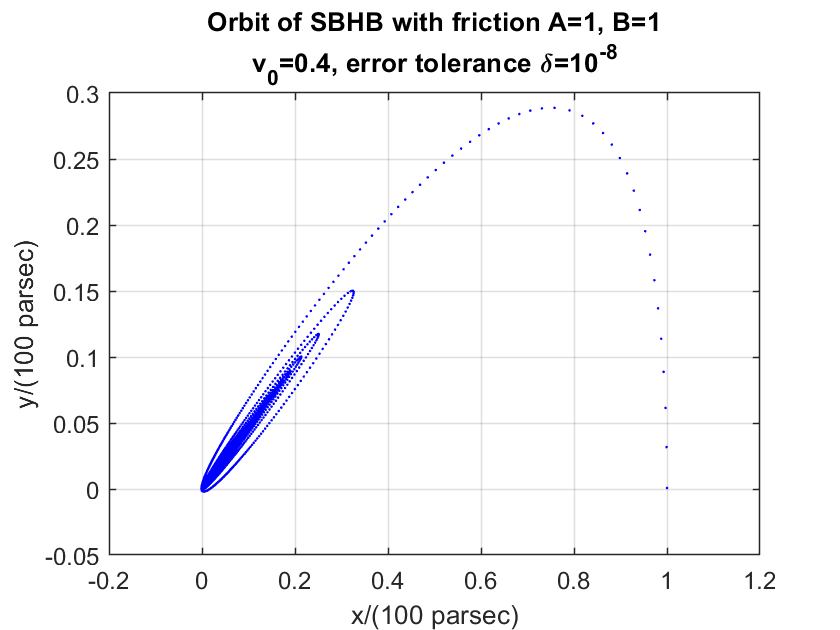
\includegraphics[width = 100mm]{BH_b8.png}
\caption{The orbit of supermassive black hole binary with dynamical friction using adaptive time step fourth-order Runge-Kutta method. Initial position $x=1$, $y=0$, constants $A=B=1$. Initial velosity $\mathbf{v}_0=(0,0.4)$, 0.8 times that of a circular orbit. Error tolerance per unit time $\delta=10^{-8}$. Two black holes keep dropping towards each other dure to friction.}
\label{fig:BHb}
\end{figure}

Fig. \ref{fig:BHb} shows that the two black holes keep dropping towards each other dure to friction, causing the radius to decrease gradually. To show the loss of energy more clearly, $\log(r)-t$ is also plotted in Fig. \ref{fig:BHblogr}. From this plot, we can imply that the perimeter radius keeps decreasing in the power law until reaching $r_S$. 

\begin{figure}[ht]
\centering
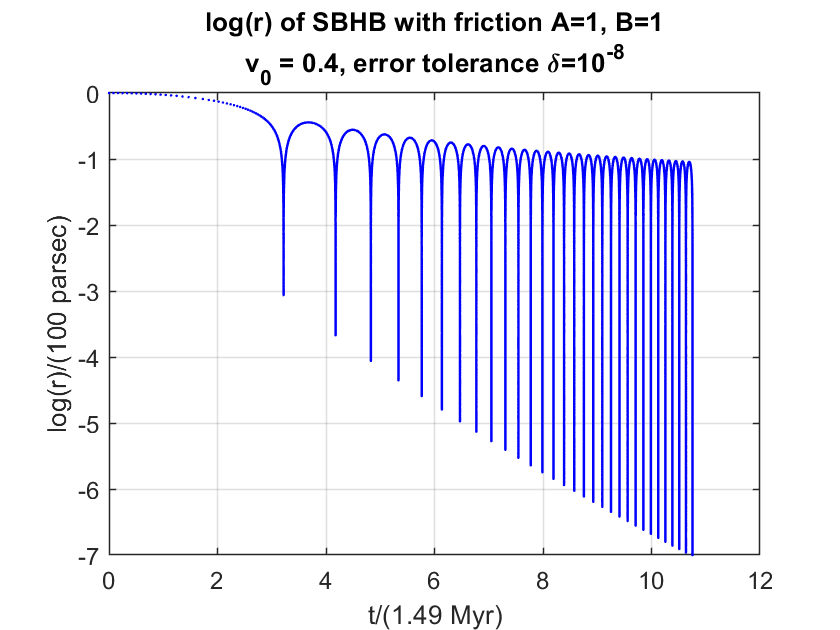
\includegraphics[width = 100mm]{BH_b8logr.png}
\caption{Logarithm of the radius of the orbit of supermassive black hole binary (SBHB) with dynamical friction using adaptive time step fourth-order Runge-Kutta method. Initial position $x=1$, $y=0$, constants $A=B=1$. Initial velosity $\mathbf{v}_0=(0,0.4)$, 0.8 times that of a circular orbit. Error tolerance per unit time $\delta=10^{-8}$. The perimeter radius keeps decreasing in the power law until reaching $r_S$. Also, the period of the cycle decrease significantly. These demonstrate that the SBHB is losing energy due to friction.}
\label{fig:BHblogr}
\end{figure}

\subsection*{c)}
When showing how the time it takes to reach the Schwarzschild radius depends on the ratio of $B/A$, to be general, $A, B$ are both chosen from 0.5 to 10 with step size of 0.5, i.e. $A, B=0.5, 1, 1.5..., 10$. Then the time to reach $r_S$ are calculated for all possible combinitions. For a small number of the combinations, the program failed to return a solution due to the large $t$ expected. For all the available data, the time is plotted with respect to the ratio of $B/A$, regardless of the individual values, and calculated for several different values of initial velocity. For $v\neq0.4$, only part of the combinations are calculated, but it does not affect showing the trend. From Fig. \ref{fig:BHc}, we can see that for the initial velocities calculated and the range of $A, B$ given, the relationship of the time it takes to reach $r_S$ and $B/A$ are quite similar. To determine exactly the relationship, a log-log plot is introduced as Fig. \ref{fig:BHclog}. Therefore, it is clearly that, for the parameters chosen, when $B/A$ is bigger or smaller than about 0.5, the time each follow a power-law rule. 

\begin{figure}[ht]
\centering
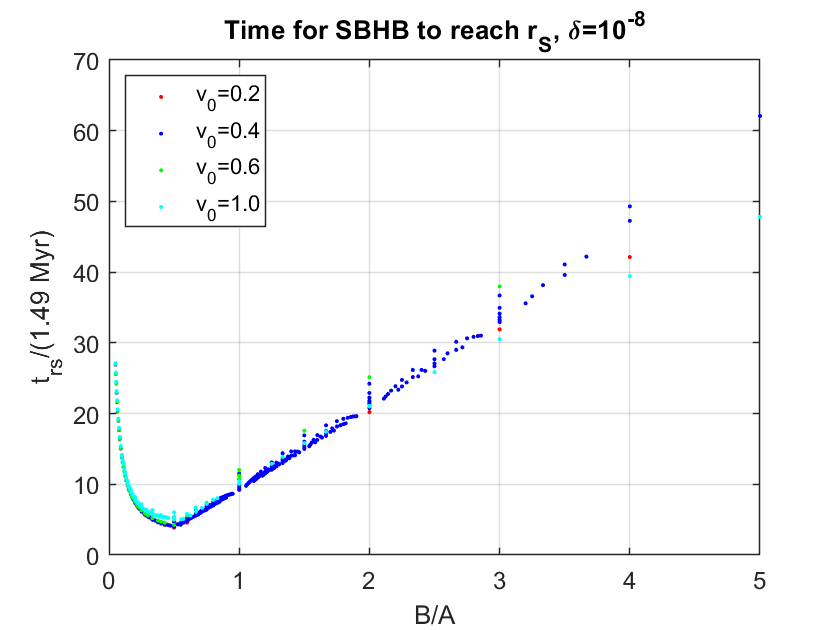
\includegraphics[width = 120mm]{trs.png}
\caption{The time it takes to reach the Schwarzschild radius with respect to the ratio of $B/A$. $A, B=0.5, 1, 1.5..., 10$. A small number of combinations failed to get a solution due to the large $t$ expected. For $v\neq0.4$, only part of the combinations are calculated. From the plot we can imply that, for the parameters chosen, the relationship of the time it takes to reach $r_S$ and $B/A$ are quite similar. The time increases rapidly when $B/A$ is large or very small}
\label{fig:BHc}
\end{figure}

\begin{figure}[ht]
\centering
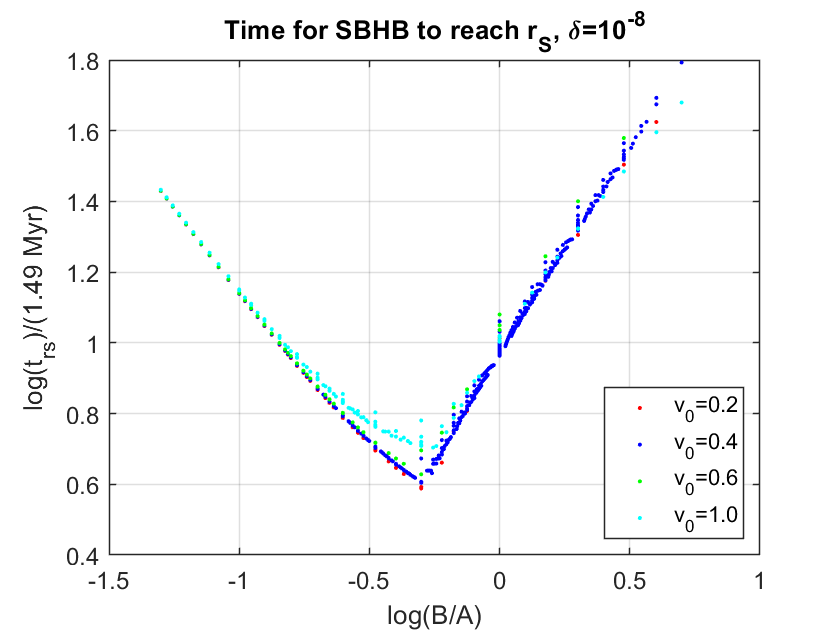
\includegraphics[width = 120mm]{trs_log.png}
\caption{The time it takes to reach the Schwarzschild radius with respect to the ratio of $B/A$. $A, B=0.5, 1, 1.5..., 10$. A small number of combinations failed to get a solution due to the large $t$ expected. For $v\neq0.4$, only part of the combinations are calculated. It is clear that within the chosen paramaters, the time and the ratio follows two different power-lows for $B/A$ larger or smaller than arround 0.5. When $v_0$ is getting larger, the relationship starts deviating power-low.}
\label{fig:BHclog}
\end{figure}

When $B/A\to 0$, the value of the dynamical friction term $|\frac{A}{v^3+B}\mathbf{v}|\to\frac{A}{v^2}$. That is, for low speed, the friction is large, and vice versa. However, take the speed plot of part a) as an example, referring to Fig. \ref{fig:BHalogv}, for the majority of time, the velocity of BH $v\ll 1$, so in this case, the friction slows down the BH significantly when $r$ is not small. \par
When $B/A\to\infty$, for small initial velocity, the cubic term in the denominator of friction can be neglected,  $|\frac{A}{v^3+B}\mathbf{v}|\to\frac{Av}{B}\to 0$. The friction is too small so that it takes a lot of time to wait until losing enough energy. 

\clearpage

\begin{figure}[ht]
\centering
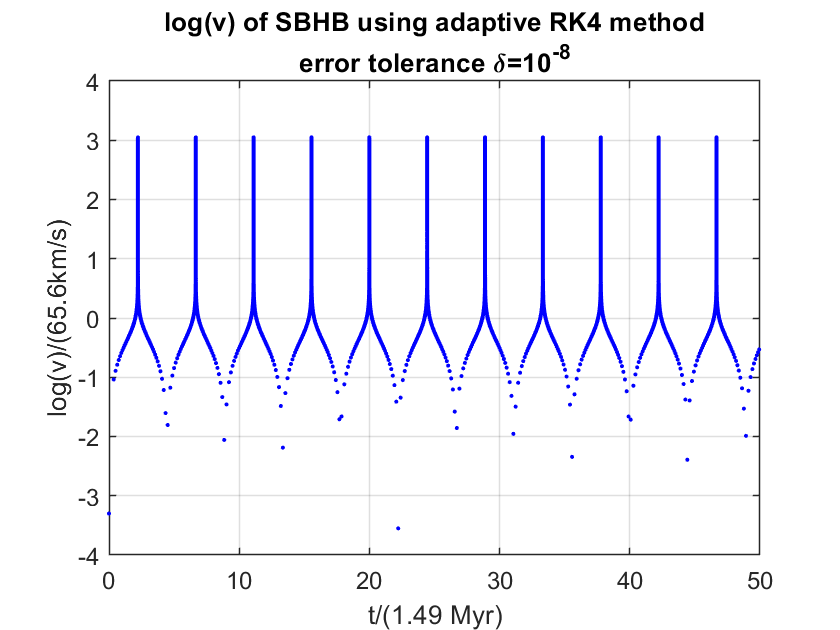
\includegraphics[width = 120mm]{BH_a8logv.png}
\caption{The velocity of supermassive black hole binary without dynamical friction using adaptive time step fourth-order Runge-Kutta method. Initial position $x=1$, $y=0$, targer time range $H=50$. Initial velosity $\mathbf{v}_0=(0,2.236\times10^{-4})$ so that the pericenter radius $r_\mathrm{peri}=r_S=10^{-7}$ is the Schwartzschild radius. From the plot we can infer that for most of the time, $v<1$. Only for very short period the velocity id extremely high.}
\label{fig:BHalogv}
\end{figure}

\subsection*{d)}
From Fig. \ref{fig:BHclog} we can easily see that the initial velocity do affect the result, since all the $A, B$'s are within the same set. Take $B/A=1$ as a example, and calculate for $v_0$ in a bigger range. In Fig. \ref{fig:trsv}, $v_0$ is covered within [0.1, 1.6], calculated for $A=B=0.5, 1.0$. It is obvious that when $v_0>1$, time grows really fast. For the range of $A, B$ given, when $v_0>1$, the cubic term in the friction cannot be neglected for much longer time. So it is similar to when $B/A\to 0$, BH gets slowed down significantly when velocity if relatively small, thus increasing the time. And how the time depends on $v_0$ relies on the exact value of $A, B$. \par

\begin{figure}[ht]
\centering
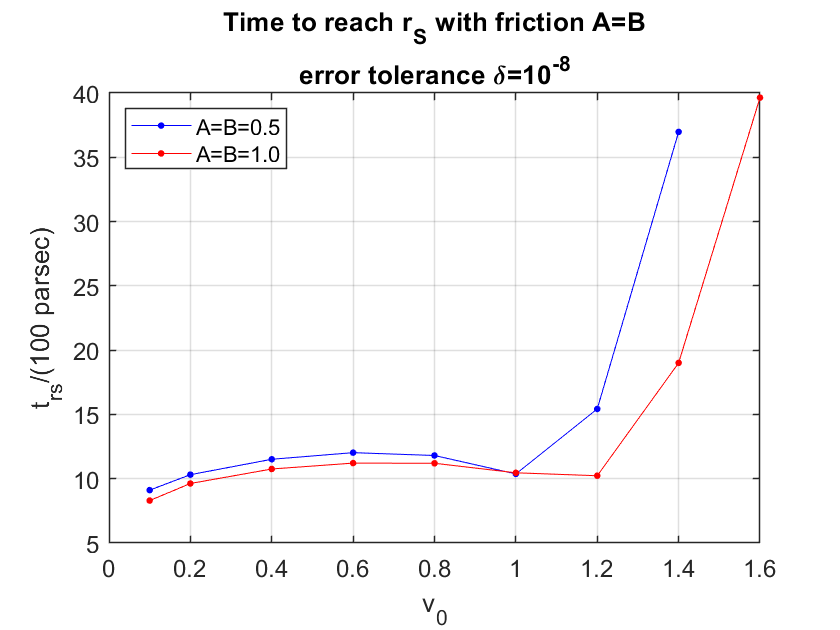
\includegraphics[width = 100mm]{trs_v.png}
\caption{The relationship of the time it takes to reach the Schwarzschild radius and the initial velocity. Constants chosen $A=B=0.5, 1.0$. $v_0\in [0.1, 1.6]$. For the $A, B$ chosen, we can see that the timw grows rapidly when $v_0>1$ or $v_0>1.2$. Therefore, the result of the time depends on the initial velosity, but the relationship also depends on the exact value of $A, B$.}
\label{fig:trsv}
\end{figure}

It can be easily implied that the result does not only depend on the ratio, but also the exact value, according to Fig. \ref{fig:BHc}, since for the same velocity and same ratio, there are still various reslts, although not quite different. Here also choose $B/A=1$ as an example, we calculate the results for different individual values for $v_0=0.4$. The results are shown in Fig. \ref{fig:trsAB}. When $A, B$ are small, for tha same ratio, the smaller the exact values are, the less likely the cubic term in friction can be neglected. Take an extrema example, when $A, B\to 0$, $|\frac{A}{v^3+B}\mathbf{v}|\to 0$, friction turns very small, thus making it much longer to reach $r_S$. Therefore, when the individual values grow higher, $|\frac{A}{v^3+B}\mathbf{v}|\to \frac{Av}{B}$ is constant, so in this process of increasing, the time will decrease and goes to a constant value, just as the plot shows.

\begin{figure}[ht]
\centering
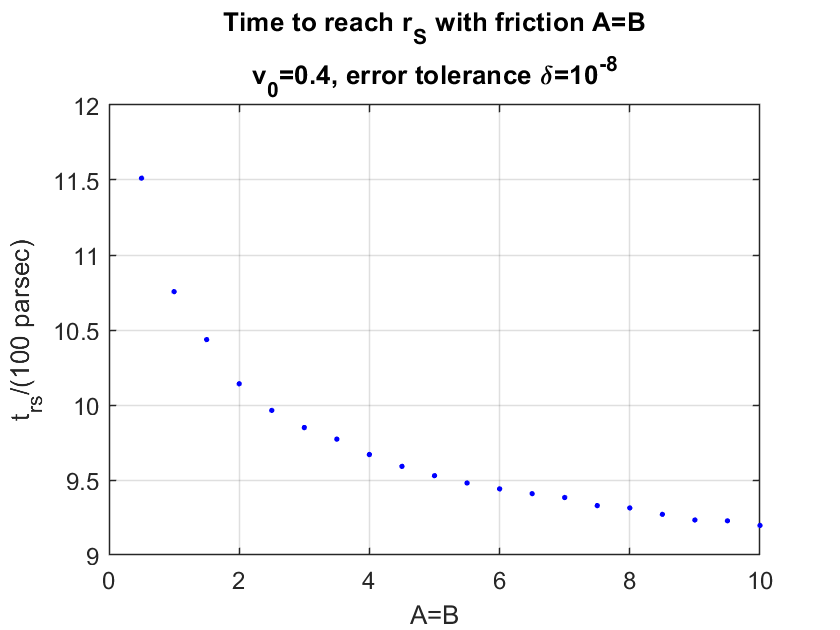
\includegraphics[width = 100mm]{trs_AB.png}
\caption{The relationship of the time it takes to reach the Schwarzschild radius and the individual value of $A, B$. Constants chosen $A=B\in[0.5, 10]$. $v_0=0.4$. For the $v_0$ and $B/A$ chosen, as the exact indivudual value increases, the time instead decreases and goes to a constant value.}
\label{fig:trsAB}
\end{figure}

\end{document}